\documentclass[titlepage,twoside,12pt]{book}

%%%%%%%%%%%%%%%%%%%%%%%%%%%%%%%%%%%%%%%%%%%%%%%%%%%%%%%%%%%%%%%%%%%%%%
% Package required for the logical manipulations
%%%%%%%%%%%%%%%%%%%%%%%%%%%%%%%%%%%%%%%%%%%%%%%%%%%%%%%%%%%%%%%%%%%%%%
\usepackage{ifthen}

%%%%%%%%%%%%%%%%%%%%%%%%%%%%%%%%%%%%%%%%%%%%%%%%%%%%%%%%%%%%%%%%%%%%%%
% AMS packages
%%%%%%%%%%%%%%%%%%%%%%%%%%%%%%%%%%%%%%%%%%%%%%%%%%%%%%%%%%%%%%%%%%%%%%
\usepackage{bm}
\usepackage{amsmath}
\usepackage{amsthm}
\usepackage{amssymb}
\usepackage{amscd}     % For simple commutative diagrams
\usepackage{stmaryrd}
\usepackage{MnSymbol}  % For \udots

\allowdisplaybreaks

%%%%%%%%%%%%%%%%%%%%%%%%%%%%%%%%%%%%%%%%%%%%%%%%%%%%%%%%%%%%%%%%%%%%%%
% Structure of the theorems, propositions, ...
%%%%%%%%%%%%%%%%%%%%%%%%%%%%%%%%%%%%%%%%%%%%%%%%%%%%%%%%%%%%%%%%%%%%%%

\usepackage[breakable]{tcolorbox}
\tcbuselibrary{skins}

\newcounter{focus}[section]
\renewcommand\thefocus{\thesection.\arabic{focus}}
\newcommand{\focuscolor}{violet}

\newenvironment{focus}[2][TTT]{%
  \refstepcounter{focus}%
  \ifthenelse{\equal{\dfn}{#2}}{\renewcommand{\focuscolor}{purple}}{%
    \ifthenelse{\equal{\alg}{#2}}{\renewcommand{\focuscolor}{red}}{%
      \ifthenelse{\equal{\cod}{#2}}{\renewcommand{\focuscolor}{yellow}}{}}}%
  \begin{tcolorbox}[enhanced,breakable,colback=\focuscolor!5!white,colframe=\focuscolor!50!white,colbacktitle=\focuscolor!50!white,coltitle=black,drop fuzzy shadow=black!50!white,title={\bfseries #2 \thefocus}%
    \ifthenelse{\equal{TTT}{#1}}{}{\ ({\bfseries #1})}]%
    \renewcommand{\labelitemi}{\textbullet}%
  }{\end{tcolorbox}}

\newenvironment{focus*}[2][TTT]{%
  \ifthenelse{\equal{\dfn}{#2}}{\renewcommand{\focuscolor}{purple}}{%
    \ifthenelse{\equal{\alg}{#2}}{\renewcommand{\focuscolor}{red}}{%
      \ifthenelse{\equal{\cod}{#2}}{\renewcommand{\focuscolor}{yellow}}{
        \ifthenelse{\equal{\qst}{#2}}{\renewcommand{\focuscolor}{black}}{}}}}%
  \begin{tcolorbox}[enhanced,breakable,colback=\focuscolor!5!white,colframe=\focuscolor!50!white,colbacktitle=\focuscolor!50!white,coltitle=black,drop fuzzy shadow=black!50!white,title={\bfseries #2}%
    \ifthenelse{\equal{TTT}{#1}}{}{\ ({\bfseries #1})}]%
    \renewcommand{\labelitemi}{\textbullet}%
  }{\end{tcolorbox}}

\newcommand{\dfn}{Definition}
\newcommand{\prp}{Proposition}
\newcommand{\thm}{Theorem}
\newcommand{\crl}{Corollary}
\newcommand{\lmm}{Lemma}
\newcommand{\alg}{Algorithm}
\newcommand{\cod}{Code}
\newcommand{\qst}{Question(s)}

\newenvironment{defn}[1][TTT]{%
\ifthenelse{\equal{TTT}{#1}}{\begin{focus}{\dfn}}{\begin{focus}[#1]{\dfn}}%
}{\end{focus}}
\newenvironment{prop}[1][TTT]{%
\ifthenelse{\equal{TTT}{#1}}{\begin{focus}{\prp}}{\begin{focus}[#1]{\prp}}%
}{\end{focus}}
\newenvironment{theorem}[1][TTT]{%
\ifthenelse{\equal{TTT}{#1}}{\begin{focus}{\thm}}{\begin{focus}[#1]{\thm}}%
}{\end{focus}}
\newenvironment{cor}[1][TTT]{%
\ifthenelse{\equal{TTT}{#1}}{\begin{focus}{\crl}}{\begin{focus}[#1]{\crl}}%
}{\end{focus}}
\newenvironment{lemma}[1][TTT]{%
\ifthenelse{\equal{TTT}{#1}}{\begin{focus}{\lmm}}{\begin{focus}[#1]{\lmm}}%
}{\end{focus}}
\newenvironment{algo}[1][TTT]{%
\ifthenelse{\equal{TTT}{#1}}{\begin{focus}{\alg}}{\begin{focus}[#1]{\alg}}%
}{\end{focus}}
\newenvironment{code}[1][TTT]{%
\ifthenelse{\equal{TTT}{#1}}{\begin{focus}{\cod}}{\begin{focus}[#1]{\cod}}%
}{\end{focus}}
\newenvironment{Quest}[1][TTT]{%
\ifthenelse{\equal{TTT}{#1}}{\begin{focus}{\qst}}{\begin{focus}[#1]{\qst}}%
}{\end{focus}}

\newenvironment{defn*}[1][TTT]{%
\ifthenelse{\equal{TTT}{#1}}{\begin{focus*}{\dfn}}{\begin{focus*}[#1]{\dfn}}%
}{\end{focus*}}
\newenvironment{prop*}[1][TTT]{%
\ifthenelse{\equal{TTT}{#1}}{\begin{focus*}{\prp}}{\begin{focus*}[#1]{\prp}}%
}{\end{focus*}}
\newenvironment{theorem*}[1][TTT]{%
\ifthenelse{\equal{TTT}{#1}}{\begin{focus*}{\thm}}{\begin{focus*}[#1]{\thm}}%
}{\end{focus*}}
\newenvironment{cor*}[1][TTT]{%
\ifthenelse{\equal{TTT}{#1}}{\begin{focus*}{\crl}}{\begin{focus*}[#1]{\crl}}%
}{\end{focus*}}
\newenvironment{lemma*}[1][TTT]{%
\ifthenelse{\equal{TTT}{#1}}{\begin{focus*}{\lmm}}{\begin{focus*}[#1]{\lmm}}%
}{\end{focus*}}
\newenvironment{algo*}[1][TTT]{%
\ifthenelse{\equal{TTT}{#1}}{\begin{focus*}{\alg}}{\begin{focus*}[#1]{\alg}}%
}{\end{focus*}}
\newenvironment{code*}[1][TTT]{%
\ifthenelse{\equal{TTT}{#1}}{\begin{focus*}{\cod}}{\begin{focus*}[#1]{\cod}}%
}{\end{focus*}}
\newenvironment{Quest*}[1][TTT]{%
\ifthenelse{\equal{TTT}{#1}}{\begin{focus*}{\qst}}{\begin{focus*}[#1]{\qst}}%
}{\end{focus*}}

%%%%%%%%%%%%%%%%%%%%%%%%%%%%%%%%%%%%%%%%%%%%%%%%%%%%%%
% With the packages  mdframed

% \usepackage{mdframed}

% \newtheoremstyle{newstyle}{\topsep}{\topsep}{\rm}{}{\bfseries}{}{\newline}{#1 #2 (#3)}
% \theoremstyle{newstyle}

% \mdfdefinestyle{mythmstyle}{leftmargin = 0pt,%
% rightmargin = 0pt,%
% skipabove = 1em,%
% skipbelow = 1em,%
% innerleftmargin = 0pt,%
% innerrightmargin = 0pt,%
% innertopmargin = 0em,%
% innerbottommargin = 0.5em,%
% linewidth = 1.5pt,%
% innerlinewidth = 0pt,%
% middlelinewidth = 0pt,%
% outerlinewidth = 0pt,%
% roundcorner = 0pt,%
% linecolor = black,%
% innerlinecolor = black,%
% middlelinecolor = black,%
% outerlinecolor = black,%
% backgroundcolor = white,%
% fontcolor = black,%
% topline = true,%
% rightline = false,%
% leftline = false,%
% bottomline = true,%
% shadow = false}

% \mdtheorem[style=mythmstyle]{theorem}{Theorem}[section]
% \mdtheorem[style=mythmstyle]{lemma}[theorem]{Lemma}
% \mdtheorem[style=mythmstyle]{defn}[theorem]{Definition}
% \mdtheorem[style=mythmstyle]{cor}[theorem]{Corollary}
% \mdtheorem[style=mythmstyle]{prop}[theorem]{Proposition}
% \mdtheorem[style=mythmstyle]{code}[theorem]{Code}
% \mdtheorem[style=mythmstyle]{algo}[theorem]{Algorithm}

%%%%%%%%%%%%%%%%%%%%%%%%%%%%%%%%%%%%%%%%%%%%%%%%%%%%%%
% With the packages  ntheorem 
%
% \usepackage[amsmath]{ntheorem}

% \theoremstyle{break}
% %\theorempostskipamount{}
% %\theorempreskipamount{}
% \theoremprework{\smallskip\rule[-1ex]{0.9\textwidth}{1pt}}
% \theorempostwork{\vspace{-1.5em}\rule{0.9\textwidth}{1pt}\newline}
% \theorembodyfont{\rm}
% \newtheorem{theorem}{Theorem}[section]

% \theoremprework{\smallskip\rule[-1ex]{0.9\textwidth}{1pt}}
% \theorempostwork{\vspace{-1.5em}\rule{0.9\textwidth}{1pt}\newline}
% \newtheorem{lemma}[theorem]{Lemma}

% \theoremprework{\smallskip\rule[-1ex]{0.9\textwidth}{1pt}}
% \theorempostwork{\vspace{-1.5em}\rule{0.9\textwidth}{1pt}\newline}
% \newtheorem{defn}[theorem]{Definition}

% \theoremprework{\smallskip\rule[-1ex]{0.9\textwidth}{1pt}}
% \theorempostwork{\vspace{-1.5em}\rule{0.9\textwidth}{1pt}\newline}
% \newtheorem{cor}[theorem]{Corollary}

% \theoremprework{\smallskip\rule[-1ex]{0.9\textwidth}{1pt}}
% \theorempostwork{\vspace{-1.5em}\rule{0.9\textwidth}{1pt}\newline}
% \newtheorem{prop}[theorem]{Proposition}

% \theoremprework{\smallskip\rule[-1ex]{0.9\textwidth}{1pt}}
% \theorempostwork{\vspace{-1.5em}\rule{0.9\textwidth}{1pt}\newline}
% \newtheorem{method}[theorem]{Method}

%%%%%%%%%%%%%%%%%%%%%%%%%%%%%%%%%%%%%%%%%%%%%%%%%%%%%%
% Without the packages  ntheorem  or  mdframed
%
% \usepackage{amsthm}
%
% \newtheoremstyle{newstyle}{\topsep}{\topsep}{\rm}{}{\bfseries}{}{\newline}{#1 #2 (#3)}
% \theoremstyle{newstyle}
% \newtheorem{theorem}{Theorem}[section]
% \newtheorem{lemma}[theorem]{Lemma}
% \newtheorem{defn}[theorem]{Definition}
% \newtheorem{cor}[theorem]{Corollary}
% \newtheorem{prop}[theorem]{Proposition}
% \newtheorem{method}[theorem]{Method}

\numberwithin{equation}{section}

%%%%%%%%%%%%%%%%%%%%%%%%%%%%%%%%%%%%%%%%%%%%%%%%%%%%%%%%%%%%%%%%%%%%%%
% Structure of the chapters, sections, ...
%%%%%%%%%%%%%%%%%%%%%%%%%%%%%%%%%%%%%%%%%%%%%%%%%%%%%%%%%%%%%%%%%%%%%%
\setcounter{secnumdepth}{3}

%%%%%%%%%%%%%%%%%%%%%%%%%%%%%%%%%%%%%%%%%%%%%%%%%%%%%%%%%%%%%%%%%%%%%%
% Format of the page
%%%%%%%%%%%%%%%%%%%%%%%%%%%%%%%%%%%%%%%%%%%%%%%%%%%%%%%%%%%%%%%%%%%%%%
\raggedbottom
\usepackage[letterpaper,lmargin=1in,height=9in,width=6.5in,twoside,top=1in]{geometry}
\setlength\parskip{1ex plus 0.3ex minus 0ex}
\setlength\parindent{3ex}

%%%%%%%%%%%%%%%%%%%%%%%%%%%%%%%%%%%%%%%%%%%%%%%%%%%%%%%%%%%%%%%%%%%%%%
% Header
%
% 1) the page number on the left followed by the title of the
%    chapter for the even numbered pages (left pages).
% 2) the page number on the right preceded by the title of the
%    section for the odd numbered pages (right pages).
% For a one-sided document, only 2 is applied.
%%%%%%%%%%%%%%%%%%%%%%%%%%%%%%%%%%%%%%%%%%%%%%%%%%%%%%%%%%%%%%%%%%%%%%
\usepackage{fancyhdr}
\pagestyle{fancy}
\setlength{\headheight}{\baselineskip}
\setlength{\headsep}{1.5\baselineskip}
\renewcommand{\chaptermark}[1]{\markboth{\thechapter.\ #1}{}}
\renewcommand{\sectionmark}[1]{\markright{\thesection.\ #1}}
\renewcommand{\headrulewidth}{0.5pt}
\renewcommand{\plainheadrulewidth}{0pt}
\fancyhf{}
\fancyhead[LE,RO]{\small\thepage}
\fancyhead[LO]{\small\rightmark}
\fancyhead[RE]{\small\leftmark}

%%%%%%%%%%%%%%%%%%%%%%%%%%%%%%%%%%%%%%%%%%%%%%%%%%%%%%%%%%%%%%%%%%%%%%
% Hyper references
%%%%%%%%%%%%%%%%%%%%%%%%%%%%%%%%%%%%%%%%%%%%%%%%%%%%%%%%%%%%%%%%%%%%%%
\usepackage[pdfa=true]{hyperref}
\hypersetup{colorlinks=true,linkcolor=blue,citecolor=blue,urlcolor=blue}

%%%%%%%%%%%%%%%%%%%%%%%%%%%%%%%%%%%%%%%%%%%%%%%%%%%%%%%%%%%%%%%%%%%%%%
% For chapters without a chapter number
%
% You will have to add after the title of the chapter the
% following commands if you want your tables to be numbered  A.1, ...
%
% \setcounter{table}{0}
% \renewcommand{\thetable}{A.\arabic{table}}
%
% Add similar commands for the number of the equations, the sections,
% etc.
%%%%%%%%%%%%%%%%%%%%%%%%%%%%%%%%%%%%%%%%%%%%%%%%%%%%%%%%%%%%%%%%%%%%%%
\newcommand{\nonumchapter}[1]{
  \chapter*{#1}
  \markboth{#1}{#1}
  \addcontentsline{toc}{chapter}{#1}
}

%%%%%%%%%%%%%%%%%%%%%%%%%%%%%%%%%%%%%%%%%%%%%%%%%%%%%%%%%%%%%%%%%%%%%%
% For sections without a number
%
% You will have to add after the title of the chapter the
% following commands if you want your equations to be numbered
% chapter_number.equation_number
% 
% \renewcommand{\theequation}{\thechapter.\arabic{equation}}
%
% Add similar commands for the number of the tables, etc.
%%%%%%%%%%%%%%%%%%%%%%%%%%%%%%%%%%%%%%%%%%%%%%%%%%%%%%%%%%%%%%%%%%%%%%
\newcommand{\nonumsection}[1]{
  \section*{#1}
  \addcontentsline{toc}{section}{#1}
}

%%%%%%%%%%%%%%%%%%%%%%%%%%%%%%%%%%%%%%%%%%%%%%%%%%%%%%%%%%%%%%%%%%%%%%
% Chapter heading for the part of the document for the solutions to
% the exercises
%%%%%%%%%%%%%%%%%%%%%%%%%%%%%%%%%%%%%%%%%%%%%%%%%%%%%%%%%%%%%%%%%%%%%%
% \makeatletter
% \newcounter{chapterS}

% \let\chapterBackup=\chapter
% \newcommand\CsolPartStart{\renewcommand\chapter{ \@afterindentfalse%
%     \secdef\Csol\sCsol}%
%   \setcounter{chapterS}{0}%
%   \renewcommand\thechapterS{\arabic{chapterS}}}

% \newcommand\Csol[2][?]{%
%   \refstepcounter{chapterS}%
%   \addcontentsline{toc}{chapter}%
%   {\protect\numberline{\thechapterS}#1}%
%   {\vspace*{2em}\noindent\large\bfseries \chaptername\ \thechapterS\quad {#2}\vspace*{1em}}%
%   \sectionmark{#1}%
%   % \@afterheading\addvspace{1em}   %  Cannot be used in horizontal mode ???
% }

% \newcommand\sCsol[1]{%
%   {\noindent\large\bfseries \chaptername\ {#1}}%
%   \@afterheading\addvspace{\baselineskip}}

% \newcommand\CsolPartEnd{\let\chapter=\chapterBackup}

% \makeatother

%%%%%%%%%%%%%%%%%%%%%%%%%%%%%%%%%%%%%%%%%%%%%%%%%%%%%%%%%%%%%%%%%%%%%%
% Table of contents, list of figures, list of tables, ...
% If your manuscript has section numbers larger than 9, many tables or
% many figures, the numbers in the table of contents, the list of tables
% or the list of figures may overlap with the titles/descriptions. This
% should solve the problem.
%%%%%%%%%%%%%%%%%%%%%%%%%%%%%%%%%%%%%%%%%%%%%%%%%%%%%%%%%%%%%%%%%%%%%%
\makeatletter
\renewcommand\l@section{\@dottedtocline{1}{1em}{4em}}
\renewcommand\l@subsection{\@dottedtocline{2}{2em}{4em}}
\renewcommand\@pnumwidth{3em}
\renewcommand\@tocrmarg{4em}
\renewcommand\l@figure[2]{\@dottedtocline{1}{1em}{4em}{#1}{#2}}
\renewcommand\l@table[2]{\@dottedtocline{1}{1em}{4em}{#1}{#2}}
\makeatother

% Stuff for the table of contents (requires titlesec because \filright, ...
% are used)
\usepackage{titlesec}
\usepackage[dotinlabels]{titletoc}

% The content label doesn't appear.  It is overwritten by something
% else.   BUG
\titlecontents{part}[0pt]{\addvspace{2em}\bfseries\titlerule[1pt]\filright}
{\contentslabel{{\large\partname\ \thecontentslabel\quad}}{1em}}
{}{\hfill\contentspage}[\addvspace{1ex}]

\titlecontents{chapter}[0pt]{\addvspace{2ex}\bfseries}
{{\large\chaptername\ \thecontentslabel\quad}}
{}{\hfill\contentspage}[\addvspace{1ex}]

\newcommand{\UOtableofcontents}{
  \tableofcontents
  \contentsfinish
  \cleardoublepage
}

\newcommand{\UOtableslist}{
  \addcontentsline{toc}{chapter}{List of Tables}
  \listoftables
  \cleardoublepage
}

\newcommand{\UOfigureslist}{
  \addcontentsline{toc}{chapter}{Table of Figures}
  \listoffigures
  \cleardoublepage
}

%%%%%%%%%%%%%%%%%%%%%%%%%%%%%%%%%%%%%%%%%%%%%%%%%%%%%%%%%%%%%%%%%%%%%%
% To produce questions and solutions for the exercises at the end of a
% chapter
%%%%%%%%%%%%%%%%%%%%%%%%%%%%%%%%%%%%%%%%%%%%%%%%%%%%%%%%%%%%%%%%%%%%%%
\newcounter{questNBR}[chapter]
\renewcommand\thequestNBR{\thechapter.\arabic{questNBR}}

\newenvironment{question}[1][TTT]{%
  \refstepcounter{questNBR}\noindent%
  {\bfseries Question \arabic{chapter}.\arabic{questNBR}}%
  \ifthenelse{\equal{TTT}{#1}}{}{\ ({\bfseries #1})} \\ \noindent}{}

\newenvironment{SOLUTION}{}{}
\newcommand{\solution}[3]{%
  \ifthenelse{\equal{#1}{show}}{%
    \begin{SOLUTION}%
      {\bfseries\noindent Question~#2}\\ #3%
    \end{SOLUTION}%
  }{}}

\newcommand{\SOL}{hide}
\newcommand{\setSOL}{\renewcommand{\SOL}{show}}

%%%%%%%%%%%%%%%%%%%%%%%%%%%%%%%%%%%%%%%%%%%%%%%%%%%%%%%%%%%%%%%%%%%%%%
% Proof environment
%%%%%%%%%%%%%%%%%%%%%%%%%%%%%%%%%%%%%%%%%%%%%%%%%%%%%%%%%%%%%%%%%%%%%%

% The filled box corresponding to the empty box suggested by the AMS
% \renewcommand{\qedsymbol}{$\blacksquare$}
% I prefer this box
\renewcommand{\qedsymbol}{\rule{0.4em}{0.7em}}

% I prefer bold characters.
\renewcommand*{\proofname}{{\normalfont\bfseries Proof}}

\makeatletter
\renewenvironment{proof}[1][\proofname]{\par\pushQED{\qed}%
\normalfont \topsep6\p@\@plus6\p@\relax
\trivlist
\item\relax {\normalfont\bfseries #1\@addpunct{.}}\newline
}{\popQED\endtrivlist\@endpefalse}
\makeatother

%%%%%%%%%%%%%%%%%%%%%%%%%%%%%%%%%%%%%%%%%%%%%%%%%%%%%%%%%%%%%%%%%%%%%%
% To be able to draw circles, ovals, ... in the picture environment.
%%%%%%%%%%%%%%%%%%%%%%%%%%%%%%%%%%%%%%%%%%%%%%%%%%%%%%%%%%%%%%%%%%%%%%
\setlength{\unitlength}{1cm}
% \usepackage[pdftex]{pict2e}

%%%%%%%%%%%%%%%%%%%%%%%%%%%%%%%%%%%%%%%%%%%%%%%%%%%%%%%%%%%%%%%%%%%%%%
% To get double angle bracket, on may use the package MnSymbol.
% However, this package conflicts with ams symbols.
% Here is the code in MnSymbol to produce \llangle and \rrangle
%%%%%%%%%%%%%%%%%%%%%%%%%%%%%%%%%%%%%%%%%%%%%%%%%%%%%%%%%%%%%%%%%%%%%%

\makeatletter
\DeclareFontFamily{OMX}{MnSymbolE}{}
\DeclareSymbolFont{MnLargeSymbols}{OMX}{MnSymbolE}{m}{n}
\SetSymbolFont{MnLargeSymbols}{bold}{OMX}{MnSymbolE}{b}{n}
\DeclareFontShape{OMX}{MnSymbolE}{m}{n}{
    <-6>  MnSymbolE5
   <6-7>  MnSymbolE6
   <7-8>  MnSymbolE7
   <8-9>  MnSymbolE8
   <9-10> MnSymbolE9
  <10-12> MnSymbolE10
  <12->   MnSymbolE12
}{}
\DeclareFontShape{OMX}{MnSymbolE}{b}{n}{
    <-6>  MnSymbolE-Bold5
   <6-7>  MnSymbolE-Bold6
   <7-8>  MnSymbolE-Bold7
   <8-9>  MnSymbolE-Bold8
   <9-10> MnSymbolE-Bold9
  <10-12> MnSymbolE-Bold10
  <12->   MnSymbolE-Bold12
}{}

\let\llangle\@undefined
\let\rrangle\@undefined
\DeclareMathDelimiter{\llangle}{\mathopen}%
                     {MnLargeSymbols}{'164}{MnLargeSymbols}{'164}
\DeclareMathDelimiter{\rrangle}{\mathclose}%
                     {MnLargeSymbols}{'171}{MnLargeSymbols}{'171}
\makeatother

%%%%%%%%%%%%%%%%%%%%%%%%%%%%%%%%%%%%%%%%%%%%%%%%%%%%%%%%%%%%%%%%%%%%%%
% Package to properly format some parts of the text
%%%%%%%%%%%%%%%%%%%%%%%%%%%%%%%%%%%%%%%%%%%%%%%%%%%%%%%%%%%%%%%%%%%%%%
\usepackage{ulem}        % To properly underline words, sentences, ...
\usepackage{url}         % To get normal url
\usepackage{verbatim}
\usepackage[margin=0.05\textwidth]{caption}

%%%%%%%%%%%%%%%%%%%%%%%%%%%%%%%%%%%%%%%%%%%%%%%%%%%%%%%%%%%%%%%%%%%%%%
% For minipage
%%%%%%%%%%%%%%%%%%%%%%%%%%%%%%%%%%%%%%%%%%%%%%%%%%%%%%%%%%%%%%%%%%%%%%
\newlength{\miniwidth}
\setlength{\miniwidth}{\textwidth}
\addtolength{\miniwidth}{-2cm}

%%%%%%%%%%%%%%%%%%%%%%%%%%%%%%%%%%%%%%%%%%%%%%%%%%%%%%%%%%%%%%%%%%%%%%
% For tables that extent over the next page.
%%%%%%%%%%%%%%%%%%%%%%%%%%%%%%%%%%%%%%%%%%%%%%%%%%%%%%%%%%%%%%%%%%%%%%
\usepackage{longtable}

%%%%%%%%%%%%%%%%%%%%%%%%%%%%%%%%%%%%%%%%%%%%%%%%%%%%%%%%%%%%%%%%%%%%%%
% For (horizontal and more) lists inside a paragraph
%%%%%%%%%%%%%%%%%%%%%%%%%%%%%%%%%%%%%%%%%%%%%%%%%%%%%%%%%%%%%%%%%%%%%%
\usepackage{paralist}

%%%%%%%%%%%%%%%%%%%%%%%%%%%%%%%%%%%%%%%%%%%%%%%%%%%%%%%%%%%%%%%%%%%%%%
% Important variables supplied by the user
%%%%%%%%%%%%%%%%%%%%%%%%%%%%%%%%%%%%%%%%%%%%%%%%%%%%%%%%%%%%%%%%%%%%%%
\newcommand{\UO}{University of Ottawa}
\newcommand{\setUO}[1]{\renewcommand{\UO}{#1}}

\newcommand{\UOfac}{Faculty of Science}
\newcommand{\setUOfac}[1]{\renewcommand{\UOfac}{#1}}

\newcommand{\UOdept}{Department of Mathematics and Statistics}
\newcommand{\setUOdept}[1]{\renewcommand{\UOdept}{#1}}

\newcommand{\UOauthor}{Benoit Dionne}     % author
\newcommand{\setUOauthor}[1]{\renewcommand{\UOauthor}{#1}}

\newcommand{\UOtitle}{Numerical Analysis} % title
\newcommand{\setUOtitle}[1]{\renewcommand{\UOtitle}{#1}}

\newcommand{\UOyear}{2023}  % year
\newcommand{\setUOyear}[1]{\renewcommand{\UOyear}{#1}}

%%%%%%%%%%%%%%%%%%%%%%%%%%%%%%%%%%%%%%%%%%%%%%%%%%%%%%%%%%%%%%%%%%%%%%
% To print today's date in Canadian format
%%%%%%%%%%%%%%%%%%%%%%%%%%%%%%%%%%%%%%%%%%%%%%%%%%%%%%%%%%%%%%%%%%%%%%
\newcommand*{\dateCAN}{\renewcommand*{\today}{%
    \ifcase\day \or
    01\or 02\or 03\or 04\or 05\or 06\or 07\or 08\or 09\or 10\or
    11\or 12\or 13\or 14\or 15\or 16\or 17\or 18\or 19\or 20\or
    21\or 22\or 23\or 24\or 25\or 26\or 27\or 28\or 29\or 30\or
    31\fi/\ifcase\month \or
    01\or 02\or 03\or 04\or 05\or 06\or 07\or 08\or 09\or 10\or
    11\or 12\fi/\number\year}}

%%%%%%%%%%%%%%%%%%%%%%%%%%%%%%%%%%%%%%%%%%%%%%%%%%%%%%%%%%%%%%%%%%%%%%
% The title page
%%%%%%%%%%%%%%%%%%%%%%%%%%%%%%%%%%%%%%%%%%%%%%%%%%%%%%%%%%%%%%%%%%%%%%
\newcommand{\UOlogoCLloc}{images/UOlogo_headCL}
                                          % Location of the logo
\newcommand{\UOlogoCLopt}{3cm}            % Options for includegraphics
\newcommand{\setUOlogoCLloc}[2]{
  \renewcommand{\UOlogoCLloc}{#1}
  \renewcommand{\UOlogoCLopt}{#2}
}

\usepackage{incgraph}
\usetikzlibrary{fadings}

\newcommand{\titlePage}{
  \thispagestyle{empty}
  \begin{titlepage}
    \newsavebox{\caversea}
    \savebox{\caversea}{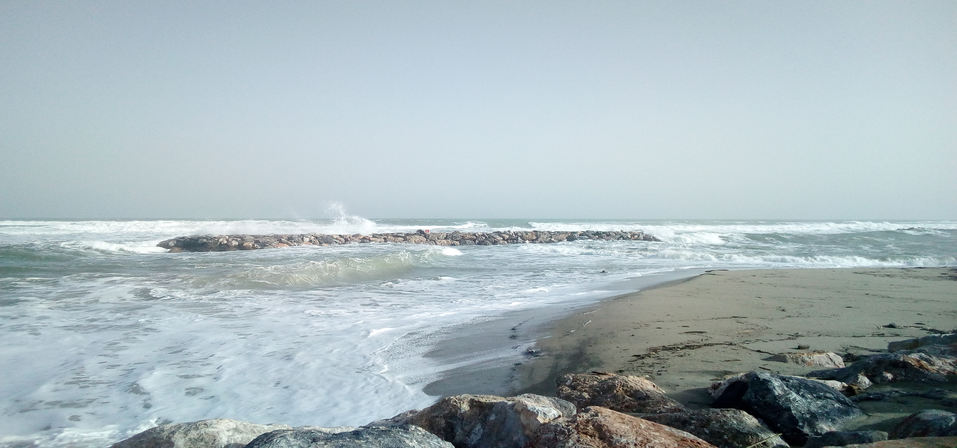
\includegraphics[width=7in]{images/cover_sea}}
    % \newsavebox{\windmill}
    % \savebox{\windmill}{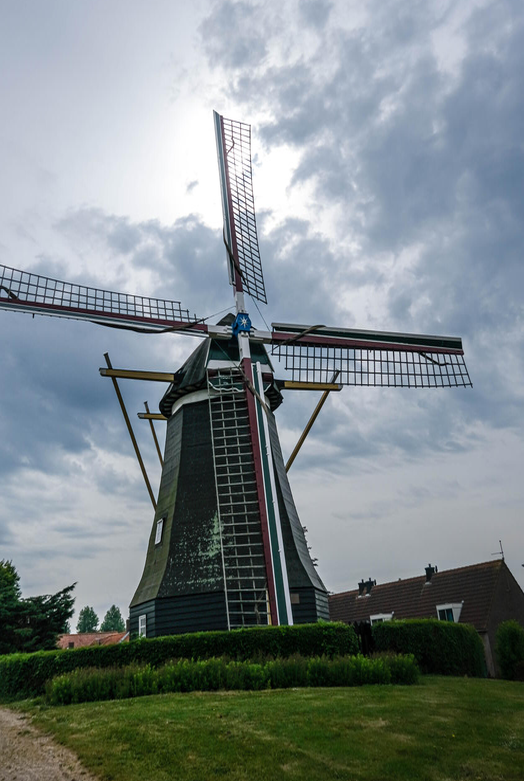
\includegraphics[width=2.5in]{images/cover_windmill}}
    \newsavebox{\bridge}
    \savebox{\bridge}{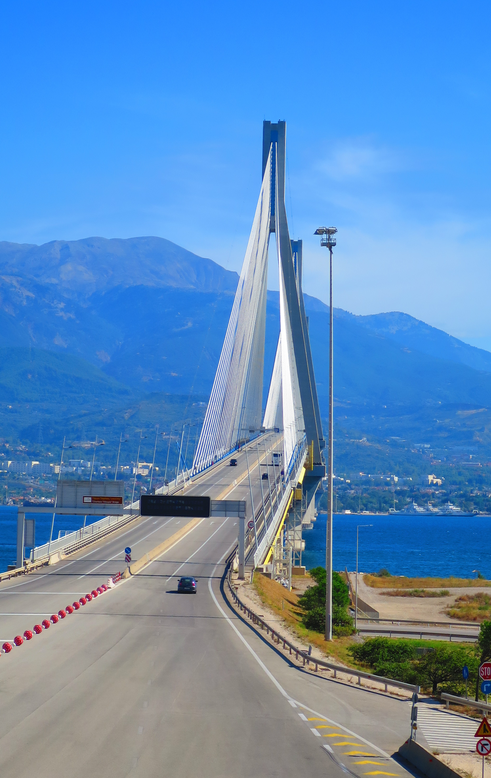
\includegraphics[width=2.5in]{images/cover_bridge}}
    \begin{inctext}[paper=current, target=mytarget]
      \begin{tikzpicture}
        \coordinate (A) at (0,0);
        \coordinate (B) at (8.5in,11in);
        \fill[use as bounding box,color=cyan!7] (A) rectangle (B);
        \coordinate (C) at ([xshift=0.5in,yshift=0.5in]A);
        \coordinate (D) at ([xshift=-0.5in,yshift=-0.5in]B);
        \draw[rounded corners=0.25in,very thick,black] (C) rectangle (D);
        \node[inner sep=0pt,above right] (sea) at (0.75in,2.5in) {\usebox{\caversea}};
        \fill[cyan!7,path fading=south] (0.75in,4.5in) rectangle (7.75in,5.8in);
        % \node[inner sep=0pt,below right] (windmill) at (0.75in,10in) {\usebox{\windmill}};
        \node[inner sep=0pt,below right] (bridge) at (0.75in,10in) {\usebox{\bridge}};
        \fill[cyan!7,path fading=north] (0.75in,6.02in) rectangle (3.3in,6.9in);
        \fill[cyan!7,path fading=west] (2.8in,6in) rectangle (3.26in,10in);
        \node[text width=10cm,align=flush center,font=\Huge\bfseries] at (5.5in,8in) {\UOtitle};
        \node[inner sep=0pt,above right] (UOlogo) at (1in,1in) {\includegraphics[width=\UOlogoCLopt]{\UOlogoCLloc}};
        \node[text width=6cm,above left,font=\large\bfseries] (author) at (7.5in,1in) {\UOauthor \\ \UO};
      \end{tikzpicture}
    \end{inctext}
  \end{titlepage}
  \pagecolor{white}
  \cleardoublepage
}

%%%%%%%%%%%%%%%%%%%%%%%%%%%%%%%%%%%%%%%%%%%%%%%%%%%%%%%%%%%%%%%%%%%%%%
% The open source page
%%%%%%%%%%%%%%%%%%%%%%%%%%%%%%%%%%%%%%%%%%%%%%%%%%%%%%%%%%%%%%%%%%%%%%
\newcommand{\UOopenloc}{images/open_source}     % Location of the logo
\newcommand{\UOopenopt}{2cm}             % Options for includegraphics

\newcommand{\opensource}{
  \thispagestyle{empty}

  \noindent \copyright\ \UOauthor, \UOyear\ (\UO)
  
  \noindent Adapted version from the notes for the courses MAT3380
  and graduate courses in numerical analysis given at the University
  of Ottawa.

  \noindent This document is available on the following sites.\\
  uO Research: \\ % http://hdl.handle.net/10393/44594 \\
  GitHub: https://github.com/BenoitDionne/Numerical\_Analysis

  \vspace*{1cm}
  
  \noindent \includegraphics[width=\UOopenopt]{\UOopenloc}

  \noindent Unless otherwise stated, this book is made available under
  the terms of the license
  \href{https://creativecommons.org/licenses/by-nc-sa/4.0/deed.en}{Creative
    Commons Attribution - Non Commercial-Share Alike 4.0 International} (CC BY-NC-SA 4.0)

  \vfill

  \noindent Cover Page:\\
  % The windmill, Netherlands, photo by Louise Oegema.\\
  The Rio–Antirio bridge, Greece, photo by Jean Dionne.\\
  The stormy Mediterranean sea, photo by Louise Oegema.

  \cleardoublepage
}

%%%%%%%%%%%%%%%%%%%%%%%%%%%%%%%%%%%%%%%%%%%%%%%%%%%%%%%%%%%%%%%%%%%%%%
% The bibliography
%%%%%%%%%%%%%%%%%%%%%%%%%%%%%%%%%%%%%%%%%%%%%%%%%%%%%%%%%%%%%%%%%%%%%%
\newcommand{\UObibliography}[1]{
  % \setcounter{chapter}{100}
  \addcontentsline{toc}{chapter}{Bibliography}
  \include{#1}
  \cleardoublepage
}

%%%%%%%%%%%%%%%%%%%%%%%%%%%%%%%%%%%%%%%%%%%%%%%%%%%%%%%%%%%%%%%%%%%%%%
% The index
%%%%%%%%%%%%%%%%%%%%%%%%%%%%%%%%%%%%%%%%%%%%%%%%%%%%%%%%%%%%%%%%%%%%%%
\usepackage{makeidx}
\makeindex
\newcommand{\UOindex}{
  \setcounter{chapter}{100}
  \addcontentsline{toc}{chapter}{\indexname}
  \printindex
}

%%%%%%%%%%%%%%%%%%%%%%%%%%%%%%%%%%%%%%%%%%%%%%%%%%%%%%%%%%%%%%%%%%%%%%
% graphics, ...
%%%%%%%%%%%%%%%%%%%%%%%%%%%%%%%%%%%%%%%%%%%%%%%%%%%%%%%%%%%%%%%%%%%%%%
\usepackage{graphicx}
\usepackage{rotating}    % To rotate figures, tables, ...
\usepackage{color}
% \usepackage{tikz}
% \usepackage{pst-node,pst-plot,auto-pst-pdf}
% \usepackage{subfig}

% By default figures will be placed "here" if possible otherwise at
% the "top."
\makeatletter
\renewcommand*{\fps@figure}{ht}
\makeatother

% Methods for jpg, png, ... figures.

\newcommand{\figbox}[2]{\begin{center}%
\includegraphics[width=#2]{#1}\end{center}}

% Methods for pdf figures.
\newcommand{\pdfbox}[1]{\begin{center}\input{#1.pdf_t}\end{center}}

\newcommand{\pdfF}[5][TTT]{%
  \ifthenelse{\equal{TTT}{#1}}{\begin{figure}}{\begin{figure}[#1]}%
      {\color{purple}\rule{\textwidth}{1pt}}\begin{center}%
        \input{#2.pdf_t}\end{center}\caption[#3]{#4 \label{#5}}%
      {\color{purple}\rule{\textwidth}{1pt}}%
    \end{figure}}

\newcommand{\pdfFD}[6][TTT]{
  \ifthenelse{\equal{TTT}{#1}}{\begin{figure}}{\begin{figure}[#1]}%
      {\color{purple}\rule{\textwidth}{1pt}}\begin{center} %
        \input{#2.pdf_t}\end{center} %
      \begin{center}\input{#3.pdf_t}\end{center} %
      \caption[#4]{#5 \label{#6}}%
      {\color{purple}\rule{\textwidth}{1pt}}%
    \end{figure}}

% Methods for png, jpg, ... figures.

\newcommand{\mathF}[6][TTT]{%
  \ifthenelse{\equal{TTT}{#1}}{\begin{figure}}{\begin{figure}[#1]}%
      {\color{purple}\rule{\textwidth}{1pt}}\begin{center} %
        \includegraphics[width=#3]{#2}\end{center} %
      \caption[#4]{#5 \label{#6}}%
      {\color{purple}\rule{\textwidth}{1pt}}%
    \end{figure}}

\newcommand{\mathFD}[7]{\begin{figure}%
    {\color{purple}\rule{\textwidth}{1pt}}\begin{center}%
      \includegraphics[width=#2]{#1}\includegraphics[width=#4]{#3}\end{center}%
    \caption[#5]{#6 \label{#7}}%
    {\color{purple}\rule{\textwidth}{1pt}}\end{figure}}

% Formats for the remarks, examples, ...
\newenvironment{rmk}[1][TTT]%
{\refstepcounter{focus} \noindent %
{\bfseries Remark \arabic{chapter}.\arabic{section}.\arabic{focus}}\ %
\ifthenelse{\equal{TTT}{#1}}{}{({\bfseries #1})}\\ \noindent %
}{\hspace*{\fill} $\spadesuit$}

\newenvironment{rmkList}%   % special case for remarks starting with a list
{\refstepcounter{focus} \noindent %
{\bfseries Remark \arabic{chapter}.\arabic{section}.\arabic{focus}}\\ %
\vspace*{-2\topskip}\noindent}%
{\vspace*{-\topskip}\hspace*{\fill} $\spadesuit$}

\newenvironment{egg}[1][TTT]{%
  \refstepcounter{focus}\noindent%
  {\bfseries Example \arabic{chapter}.\arabic{section}.\arabic{focus}}\ %
  \ifthenelse{\equal{TTT}{#1}}{}{({\bfseries #1})}\\ \noindent %
}{\hspace*{\fill} $\clubsuit$}

\newenvironment{eggList}[1][TTT]{ % special case for ex. starting with a list
  \refstepcounter{focus}\noindent%
  {\bfseries Example \arabic{chapter}.\arabic{section}.\arabic{focus}}\ %
  \ifthenelse{\equal{TTT}{#1}}{}{ ({\bfseries #1})} \\ %
  \vspace*{-2\topskip} \noindent %
}{\vspace*{-\topskip}\hspace*{\fill} $\clubsuit$}

% Title for the multiple choices, the parts of a proof, etc.
\newcommand{\subQ}[1]{\noindent {\bfseries #1})\ }
\newcommand{\subI}[1]{\noindent {\bfseries #1}:\ }
\newcommand{\stage}[1]{\noindent {\bfseries #1}) \ }

%%%%%%%%%%%%%%%%%%%%%%%%%%%%%%%%%%%%%%%%%%%%%%%%%%%%%%%%%%%%%%%%%%%%%%
% Mathematical symbols, short cuts, ...
%%%%%%%%%%%%%%%%%%%%%%%%%%%%%%%%%%%%%%%%%%%%%%%%%%%%%%%%%%%%%%%%%%%%%%
\newcommand{\NN}{\mathbb{N}}
\newcommand{\NNp}{\mathbb{N}^+}
\newcommand{\ZZ}{\mathbb{Z}}
\newcommand{\RR}{\mathbb{R}}
\newcommand{\QQ}{\mathbb{Q}}
\newcommand{\CC}{\mathbb{C}}

\newcommand{\BB}{\mathcal{B}}   % Denotes an atlas for a manifold
\newcommand{\EE}{\mathcal{E}}
\newcommand{\FF}{\mathcal{F}}
\newcommand{\GG}{\mathcal{G}}
\newcommand{\LL}{\mathcal{L}}   % For linear space of bounded operators, ...
\newcommand{\KK}{\mathcal{K}}   % For linear space of compact operators, ...
\renewcommand{\SS}{\mathcal{S}} % For schwartz rapidly decreasing functions, ..
\newcommand{\DD}{\mathcal{D}}   % For the test functions, ...
\newcommand{\DO}{\mathcal{D}}   % For the domain of a function, ...
\newcommand{\B}{\mathcal{B}}
\newcommand{\D}{\mathcal{D}}
\newcommand{\E}{\mathcal{E}}
\newcommand{\F}{\mathcal{F}}
\newcommand{\Q}{\mathcal{Q}}
\newcommand{\U}{\mathcal{U}}
\newcommand{\X}{\mathcal{X}}
\newcommand{\Y}{\mathcal{Y}}
\newcommand{\MM}{\mathcal{M}}
\newcommand{\OO}{\mathcal{O}}
\newcommand{\PP}{\mathcal{P}}
\newcommand{\IMG}{\mathcal{R}}      % For the range of a function, ...
\newcommand{\KE}{\mathcal{N}}       % For the kernel of a function, ...
\newcommand{\GR}{\mathcal{G}}       % For the graph of a function, ...
\newcommand{\HW}{H_{\VEC{w}}}

\DeclareMathOperator*{\esssup}{ess\;sup}
\DeclareMathOperator*{\essinf}{ess\;inf}
\DeclareMathOperator{\arcsec}{arcsec}
\DeclareMathOperator{\tr}{tr}
\DeclareMathOperator{\Id}{Id}
\DeclareMathOperator{\sgn}{sgn}
% \DeclareMathOperator{\diff}{D}
\newcommand{\diff}{\mathrm{D}}
\DeclareMathOperator{\supp}{supp}
\DeclareMathOperator{\curL}{curl}
\DeclareMathOperator{\diV}{div}
\DeclareMathOperator{\graD}{\nabla}
\DeclareMathOperator{\rank}{rank}
\DeclareMathOperator{\RE}{Re}      % For the real part of a number, ...
\DeclareMathOperator{\IM}{Im}      % For the imaginary par of a number, ...
\DeclareMathOperator{\Fix}{Fix}
\DeclareMathOperator{\Per}{Per}
\DeclareMathOperator{\sep}{sep}    % For the section on ``Melnikov
                                   % Function'', file melnikov.tex
\DeclareMathOperator{\Span}{span}
\DeclareMathOperator{\diam}{diam}

\newcommand{\VEC}[1]{\mathbf{#1}}
\newcommand{\ps}[2]{ \left\langle{#1} , {#2}\right\rangle }
\newcommand{\conj}[1]{\overline{#1}}
\newcommand{\HH}{$H_{\VEC{w}}$}
\newcommand{\AP}{AP}
\newcommand{\SN}[1]{\mathrm{S}_{#1}}
\newcommand{\Sone}{S^1}
\newcommand{\torus}[1]{\mathbf{T}^{#1}}
\newcommand{\dist}[2]{\mathrm{dist}\left(#1,#2\right)}
\newcommand{\sgm}[1]{\overline{#1}}
\newcommand{\ii}{\VEC{i}}
\newcommand{\jj}{\VEC{j}}
\newcommand{\kk}{\VEC{k}}
\newcommand{\nn}{$n\times n$\ }
\newcommand{\nm}[2]{${#1}\times{#2}$\ }
\newcommand{\intpt}[1]{\lfloor{#1}\rfloor}

\newcommand{\dx}[1]{\,\mathrm{d}#1}
\newcommand{\dydx}[2]{\frac{\mathrm{d}#1}{\mathrm{d}{#2}}}
\newcommand{\dydxn}[3]{\frac{\mathrm{d}^{#3}{#1}}{\mathrm{d}{#2}^{#3}}}
\newcommand{\dfdx}[2]{\frac{\mathrm{d}}{\mathrm{d}{#2}}{#1}}
\newcommand{\dfdxn}[3]{\frac{\mathrm{d}^{#3}}{\mathrm{d}{#2}^{#3}}{#1}}

\newcommand{\pdydx}[2]{\frac{\partial{#1}}{\partial{#2}}}
\newcommand{\pdydxn}[3]{\frac{\partial^{#3}{#1}}{\partial{#2}^{#3}}}
\newcommand{\pdydxnm}[6]{\frac{\partial^{#4}{#1}}%
{\partial{#2}^{#5} \partial{#3}^{#6}}}
\newcommand{\pdydxdots}[8]{\frac{\partial^{#5}#1}%
{\partial{#2}^{#6} \partial{#3}^{#7} \ldots \partial{#4}^{#8}}}

\newcommand{\pdfdx}[2]{\frac{\partial}{\partial{#2}}{#1}}
\newcommand{\pdfdxn}[3]{\frac{\partial^{#3}}{\partial{#2}^{#3}}{#1}}
\newcommand{\pdfdxnm}[6]{\frac{\partial^{#4}}%
{\partial{#2}^{#5} \partial{#3}^{#6}}{#1}}

\newcommand{\fdiff}[2]{\mathrm{D}^{#2}{#1}}

\newcommand{\dtx}[1]{\Delta{#1}}
\newcommand{\dtxn}[2]{\Delta^{#1}{#2}}

\DeclareMathOperator{\fl}{fl}
\DeclareMathOperator{\Bot}{\,\bot\,}
\newcommand{\tildev}[1]{\tilde{\VEC{#1}}}
\newcommand{\pps}[2]{\left\llangle{#1} , {#2}\right\rrangle }
                                                       % pseudo scalar product

% For the section of Fast Fourier Transform
\newcommand{\fct}[1]{\mathbf{#1}}
\newcommand{\fctt}[1]{\tilde{\mathbf{#1}}}

\newcommand{\NNN}{\mathcal{N}}
\newcommand{\GL}[1]{\mathrm{GL}(#1)}

%%%%%%%%%%%%%%%%%%%%%%%%%%%%%%%%%%%%%%%%%%%%%%%%%%%%%%%%%%%%%%%%%%%%%%
% Trouble
%%%%%%%%%%%%%%%%%%%%%%%%%%%%%%%%%%%%%%%%%%%%%%%%%%%%%%%%%%%%%%%%%%%%%%
\newcommand{\MORE}{\begin{center}\fbox{\color{red}\bfseries TO BE COMPLETED}\end{center}}
\newcommand{\BUG}{\begin{center}\fbox{\color{red}\bfseries TO BE FIXED}\end{center}}
